\documentclass[12pt,a4paper]{report}
\usepackage[italian]{babel}
\usepackage[utf8]{inputenc}
\usepackage{parskip}        % fa in modo che ogni paragrafo sia spaziato e non abbia l'indentazione
\usepackage{hyperref}       % Per gestire i collegamenti ipertestuali
\usepackage{listings} % Pacchetto per il codice
\usepackage{xcolor} % Opzionale, per colorare il codice e le tabelle
\lstset{
  language=C++,             % Linguaggio
  basicstyle=\ttfamily,      % Stile del testo
  keywordstyle=\color{blue}, % Colore delle parole chiave
  commentstyle=\color{gray}, % Colore dei commenti
  stringstyle=\color{red},   % Colore delle stringhe
  numbers=left,              % Numeri di riga a sinistra
  numberstyle=\tiny,         % Stile dei numeri di riga
  stepnumber=1,              % Mostra un numero di riga per ogni riga
  breaklines=true,           % Spezza automaticamente le righe lunghe
  frame=single,              % Cornice attorno al codice
  tabsize=4                  % Imposta la dimensione del tab
}

\usepackage{amsmath,amssymb,amsthm}
\usepackage{fancyhdr}
\usepackage{indentfirst}
\usepackage{microtype}
\usepackage{mathrsfs}
\usepackage{setspace}
\usepackage{graphicx}  % Serve per le immagini
\usepackage{float}
\usepackage{subfigure}
\usepackage{subcaption}

\usepackage{colortbl}  % Permette di colorare degli elementi
\usepackage{booktabs}  % Migliora l'aspetto delle tabelle
\usepackage{multirow}  % Serve per unire più righe in una tabella

\graphicspath{ {./images/} }
\newcommand{\sign}{\text{sign}}

\hypersetup{
    colorlinks=true,
    linkcolor=black,
    urlcolor=blue,
    pdftitle={La metodologia di apprendimento automatico SVM per la regressione: applicazione al problema del testo sfocato},
    pdfpagemode=FullScreen,
    }

\newcommand{\omgv}{\overrightarrow{\omega}}
\newcommand{\xv}{\overrightarrow{x}}
\newcommand{\uv}{\overrightarrow{u}}
\newcommand{\xvo}{\overrightarrow{x_O}}
\newcommand{\xvx}{\overrightarrow{x_X}}
\newcommand{\xvi}{\overrightarrow{x_i}}
\newcommand{\xvj}{\overrightarrow{x_j}}

\begin{document}

\begin{titlepage}
\begin{center}
{{\Large{\textsc{Università degli Studi \\ \vspace{2mm} di Modena e Reggio Emilia}}}} \rule[0.1cm]{14cm}{0.1mm}
\rule[0.5cm]{14cm}{0.6mm}
{\small{\bf DIPARTIMENTO DI SCIENZE FISICHE, INFORMATICHE E MATEMATICHE\\
Corso di Laurea in Informatica}}

\end{center}
\vspace{20mm}
\begin{center}
{\LARGE{\bf Accelerazione di algoritmi di Stereo Matching su GPU per sistemi SLAM  }}\\
\vspace{3mm}
\end{center}
\vspace{40mm}
\par
\noindent
\begin{minipage}[t]{0.47\textwidth}
{\large{\bf Relatore:\\Dott. Filippo Muzzin}} \\
{\large{\bf Corelatore:\\Prof. Nicola Capodieci}}
\end{minipage}
\hfill
\begin{minipage}[t]{0.47\textwidth}\raggedleft
{\large{\bf Tesi di Laurea di:\\
Luca Anzaldi}}
\end{minipage}
\vspace{20mm}
\begin{center}
{\large{\bf Anno Accademico 2023/2024}}
\end{center}
\end{titlepage}

\tableofcontents

\chapter{Introduzione}

L’evoluzione delle tecnologie informatiche ha portato a una crescente necessità di eseguire calcoli complessi in tempi ridotti, specialmente nei settori che richiedono grandi potenze computazionali come la grafica, l'intelligenza artificiale e la simulazione scientifica. Per far fronte a queste esigenze, si sono sviluppati linguaggi e framework specifici per la programmazione parallela, che permettono di sfruttare le capacità di elaborazione simultanea di più core o unità di calcolo.

Questa tesi si propone di analizzare e implementare un percorso di ottimizzazione per un algoritmo di \textbf{Stereo Matching} utilizzando la tecnologia \textbf{CUDA} (Compute Unified Device Architecture), sviluppata da NVIDIA per l'elaborazione parallela su GPU. Il problema del Stereo Matching è una delle questioni fondamentali nel campo della visione artificiale e consiste nel calcolare la disparità tra due immagini catturate da punti di vista leggermente diversi (come accade negli occhi umani) al fine di ricostruire la profondità e ottenere una rappresentazione tridimensionale della scena.

Gli algoritmi di \textbf{Stereo Matching} tipicamente richiedono un'intensa capacità di calcolo, soprattutto quando si cerca di ottenere risultati accurati su immagini ad alta risoluzione. L’obiettivo principale di questa tesi è ottimizzare l'esecuzione di uno di questi algoritmi sfruttando le caratteristiche dell'elaborazione parallela offerta dalle GPU tramite CUDA. La scelta di utilizzare \textbf{CUDA} è motivata dalla sua capacità di distribuire il carico computazionale su un numero elevato di core, rendendo possibile l’elaborazione simultanea di grandi quantità di dati, e migliorando significativamente le prestazioni rispetto all'implementazione su \textbf{CPU tradizionali}.

Nella trattazione verrà esaminato l'approccio usato per ottimizare l'algoritmo  , con un'attenzione particolare all'efficienza e alla precisione, e si approfondiranno i principi di ottimizzazione parallela, analizzando tecniche come la decomposizione del problema in thread e la gestione ottimale della memoria della \textbf{GPU}. La tesi illustrerà anche i vantaggi e le sfide nell'implementare un algoritmo di Stereo Matching su architettura parallela, discutendo sia gli aspetti teorici che quelli pratici, con test sperimentali che metteranno a confronto le performance dell'algoritmo ottimizzato rispetto a versioni non parallele o meno efficienti.



\chapter{Panoramica dei linguaggi paralleli e specifiche di CUDA}

\section{Introduzione}

La programmazione parallela si basa sull’esecuzione contemporanea di più istruzioni o blocchi di codice, sfruttando risorse hardware multiprocessore, multicore o acceleratori come le GPU (\textbf{Graphics Processing Units}). A differenza della programmazione sequenziale tradizionale, che esegue le istruzioni una dopo l’altra, la programmazione parallela permette di dividere i problemi in sottoproblemi più piccoli, i quali possono essere risolti simultaneamente, aumentando l’efficienza complessiva del sistema.

Uno dei linguaggi di programmazione parallela più diffusi è \textbf{CUDA} (Compute Unified Device Architecture), un framework sviluppato da \textit{NVIDIA}.    Esso consente di sfruttare la potenza delle GPU per eseguire calcoli ad alte prestazioni, trasformando le unità grafiche in potenti strumenti di elaborazione general-purpose. Attraverso CUDA, gli sviluppatori possono scrivere codice in \textbf{C}, \textbf{C++} o Python, che viene successivamente parallelizzato e distribuito tra le varie unità di calcolo della GPU.

Inoltre, esistono altri linguaggi e API orientati alla programmazione parallela, come OpenCL, che offre un approccio più generalista e multi-piattaforma, permettendo di sfruttare anche altre tipologie di hardware, come \textbf{CPU} e \textbf{FPGA}. Questi strumenti sono oggi fondamentali per affrontare i carichi di lavoro che richiedono un’enorme quantità di calcoli in tempi contenuti, portando significativi benefici in campi come il machine learning, la crittografia, l’elaborazione video e le simulazioni fisiche.

\section{Differenza di architettura tra CPU e GPU}

L'architettura della CPU e della GPU può essere confrontata in maniera sintetica. La CPU è progettata per ridurre la latenza, ossia cerca di ottenere i risultati delle operazioni nel minor tempo possibile. Per fare questo, dispone di \textbf{cache L1} di grandi dimensioni, che aiutano a ridurre la latenza media dei dati, e utilizza poche unità logiche aritmetiche ad alte prestazioni per calcolare velocemente i risultati. I modelli moderni di CPU sfruttano anche il parallelismo a livello di istruzione, elaborando in anticipo risultati parziali per ridurre ulteriormente i tempi di attesa. Al contrario, l'architettura della GPU è orientata al \textbf{throughput}, ovvero al volume di operazioni elaborate simultaneamente. Poiché contiene un numero elevato di processori paralleli, non può dotarli di cache L1 grandi come quelle delle CPU. Di conseguenza, gli accessi alla memoria sono più lenti, causando maggiori latenze. Tuttavia, quando la GPU esegue molti più thread rispetto ai suoi core fisici (situazione chiamata “\textit{over-subscription}”), riesce a nascondere queste latenze passando rapidamente l'esecuzione da un thread all'altro.


\begin{figure}[h]
    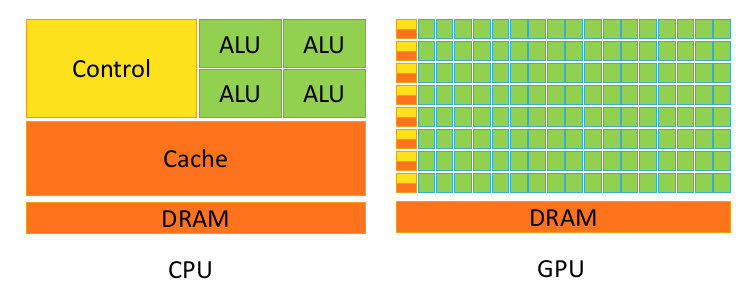
\includegraphics[width=1\linewidth]{img/CPUvsGPU.png}
    \caption{Differenza di architettura \cite{CUDAtutorial}}
\end{figure}

I \textbf{thread} della GPU sono molto più leggeri rispetto a quelli della CPU, il che rende più efficiente il loro passaggio da uno all'altro. Anche se le latenze possono essere più elevate, la capacità di commutare rapidamente i thread e di gestire più istruzioni in parallelo permette alla GPU di mantenere un \textbf{throughput elevato} durante l'elaborazione. Pertanto, i vantaggi di utilizzare le GPU per calcoli intensivi aumentano all'aumentare del numero di thread impiegati per un determinato compito.

\section{Il modello di esecuzione di CUDA}

Nel modello di esecuzione di CUDA esistono due tipi di funzioni principali:

\begin{itemize}
    \item \texttt{\_\_global\_\_}: Queste funzioni sono chiamate \textit{kernel functions} e possono essere invocate dalla \textit{host} (CPU) per essere eseguite sulla \textit{device} (GPU). Sono definite con il qualificatore \texttt{\_\_global\_\_} e devono essere invocate con una sintassi speciale, specificando il numero di thread e blocchi da lanciare. Una caratteristica particolare delle funzioni \texttt{\_\_global\_\_} è che il loro tipo di ritorno deve essere sempre \texttt{void}. Ecco un esempio di dichiarazione di una funzione \texttt{\_\_global\_\_}:

    \begin{lstlisting}
    __global__ void myKernel(int *data) {
        // Codice da eseguire sulla GPU
    }
    \end{lstlisting}

    \item \texttt{\_\_device\_\_}: Queste funzioni possono essere chiamate solo da altre funzioni eseguite sulla \textit{device} (ovvero dalla GPU stessa) e non possono essere invocate direttamente dalla \textit{host}. Le funzioni \texttt{\_\_device\_\_} sono eseguite sulla GPU e possono avere qualsiasi tipo di ritorno. Ecco un esempio di dichiarazione di una funzione \texttt{\_\_device\_\_}:

    \begin{lstlisting}
    __device__ int square(int x) {
        return x * x;
    }
    \end{lstlisting}
\end{itemize}

\begin{figure}[h]
    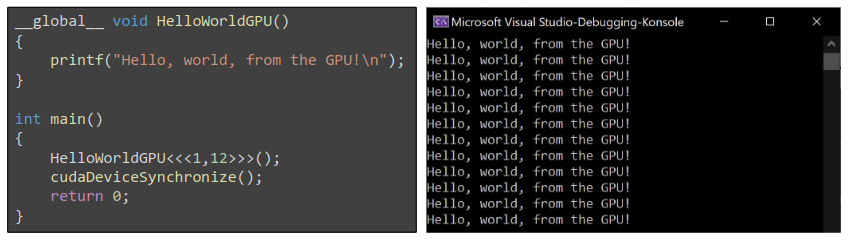
\includegraphics[width=1\linewidth]{img/basic_kernel.png}
    \caption{Kernel di base (1 blocco, 12 thread) \cite{CUDAtutorial}}
\end{figure}

\section{Sincronizzazione}

Di base, CUDA presume che, se una funzione può dipendere da un'altra, tale dipendenza sarà garantita. Pertanto, CUDA gestisce la sincronizzazione tra le diverse funzioni per assicurare che vengano eseguite nell'ordine corretto.
Ecco alcuni esempi:

\begin{itemize}
    \item Il kernel B è successivo al kernel A. Allora il kernel B aspetterà che il primo kernel abbia finito l'esecuzione.
    \item Se stiamo scrivendo i dati sulla GPU il compilatore aspetterà a lanciare la funzione di tipo \texttt{\_\_kernel\_\_}.
    \item Se vogliamo scrivere i dati dalla GPU \(\rightarrow\) CPU il compilatore aspetterà che la funzione di tipo \texttt{\_\_kernel\_\_} sia terminata.
\end{itemize}

\vspace{8mm}
\hrule
\vspace{3mm}

È possibile ovviamente sincronizzare manualmente l'esecuzione in un programma CUDA, in modo tale da controllare l'ordine di esecuzione tra kernel, thread o tra operazioni tra CPU e GPU.  I principali metodi di sincronizzazione sono i seguenti:

\begin{itemize}
    \item \textbf{Sincronizzazione tra Host e Device:}
    \begin{itemize}
        \item \texttt{cudaDeviceSynchronize()}: Questa funzione viene chiamata dalla CPU per aspettare che tutte le operazioni precedenti lanciate sulla GPU siano completate. Viene utilizzata per assicurarsi che il kernel abbia terminato l'esecuzione prima di continuare con altre operazioni sul codice host.
    \end{itemize}
    
    \item \textbf{Sincronizzazione tra Thread di un Kernel:}
    \begin{itemize}
        \item \texttt{\_\_syncthreads()}: Questa funzione viene chiamata all'interno di un kernel e sincronizza tutti i thread all'interno di un blocco. Ogni thread deve raggiungere il punto in cui è presente \texttt{\_\_syncthreads()} prima di poter proseguire, ed è utile quando c'è bisogno che tutti i thread completino un’operazione comune prima di procedere ulteriormente. Va notato che \texttt{\_\_syncthreads()} funziona solo all'interno di un singolo blocco di thread, non tra diversi blocchi.
    \end{itemize}
    
    \item \textbf{Stream e Eventi per Sincronizzazione Personalizzata:}
    \begin{itemize}
        \item CUDA supporta l'uso di stream e eventi per una sincronizzazione più avanzata. Gli stream permettono di lanciare kernel in modo asincrono e indipendente tra loro, mentre gli eventi vengono utilizzati per sincronizzare l'esecuzione tra diversi stream o per misurare il tempo di esecuzione tra operazioni.
    \end{itemize}
\end{itemize}

\section{Gerarchia di esecuzione di CUDA}

La gerarchia di esecuzione in CUDA si basa su un'architettura parallela organizzata in livelli, che consente di suddividere il lavoro complessivo in unità più piccole. Il codice viene eseguito in parallelo su molte unità di calcolo, con la possibilità di gestire grandi quantità di operazioni simultaneamente. Questa struttura permette di scalare l'esecuzione in base alle esigenze, ottimizzando l'uso delle risorse disponibili per migliorare le prestazioni complessive.

\begin{figure}[h]
    \centering
    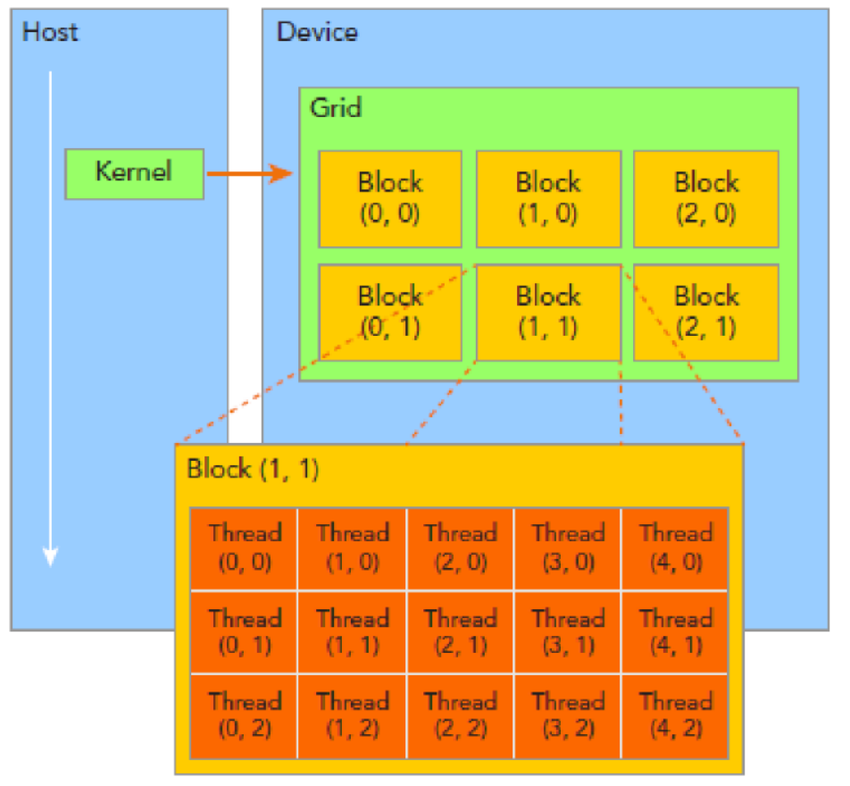
\includegraphics[width=0.7\linewidth]{img/hierarchy.png}
    \caption{Illustrazione della gerarchia di esecuzione di CUDA \cite{CUDAhierarchy}}
\end{figure}

\subsection*{Thread}
Il \textit{thread} è l'unità di base di esecuzione in CUDA. Ogni thread esegue un'istanza del codice definito in un \textit{kernel}. I thread possono essere identificati tramite un identificatore univoco (\texttt{threadIdx}) che li distingue dagli altri all'interno del loro \textit{block}.

\begin{figure}[h]
    \centering
    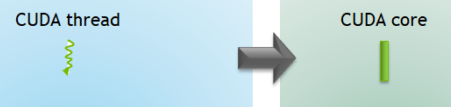
\includegraphics[width=0.7\linewidth]{img/cuda_thread.png}
    \caption{Thread nel modello di CUDA \cite{CUDA_blog}}
\end{figure}

\subsection*{Block}
I thread sono organizzati in \textit{block}, che rappresentano un gruppo di thread che può essere eseguito insieme sulla GPU. Ogni block è indipendente dagli altri, e ogni thread all'interno di un block è identificato da un indice (\texttt{threadIdx}). La dimensione massima di un block dipende dall'architettura della GPU, ma tipicamente contiene fino a 1024 thread. L'indice del block all'interno della griglia è fornito da \texttt{blockIdx}.

\begin{figure}[h]
    \centering
    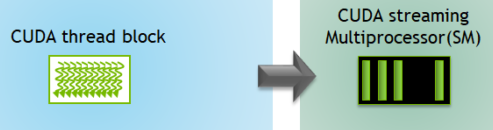
\includegraphics[width=0.7\linewidth]{img/cuda_block.png}
    \caption{Blocco(block) nel modello di CUDA \cite{CUDA_blog}}
\end{figure}



\subsection*{Grid}
I block sono organizzati in una \textit{grid}. Una grid è una collezione di block, e la dimensione della grid è determinata al momento del lancio del kernel. L'indice del block nella grid è indicato da \texttt{blockIdx}, che permette ai block di essere distinti e indirizzati individualmente.

\begin{figure}[h]
    \centering
    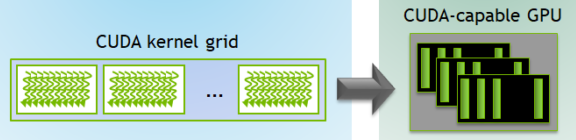
\includegraphics[width=0.7\linewidth]{img/cuda_grid.png}
    \caption{Griglia(grid) nel modello di CUDA \cite{CUDA_blog}}
\end{figure}



\subsection*{Warp}
Un concetto fondamentale nella gerarchia di esecuzione di CUDA è il \textit{warp}. Un warp è un insieme di \textbf{32 thread} che vengono eseguiti in parallelo all'interno di un singolo block. La GPU esegue i thread in gruppi di warp, e tutti i thread di un warp seguono lo stesso percorso di esecuzione (flusso di controllo), il che significa che i thread all'interno di un warp sono soggetti a esecuzione sincrona. Se i thread di un warp prendono percorsi diversi (ad esempio in caso di branch divergenti), la GPU eseguirà i percorsi separatamente, riducendo l'efficienza.



\section{Tipi di memoria}

Nell'architettura CUDA, esistono diversi tipi di memoria, ognuno con caratteristiche specifiche in termini di accesso, latenza e visibilità.


\begin{figure}[h]
    \centering
    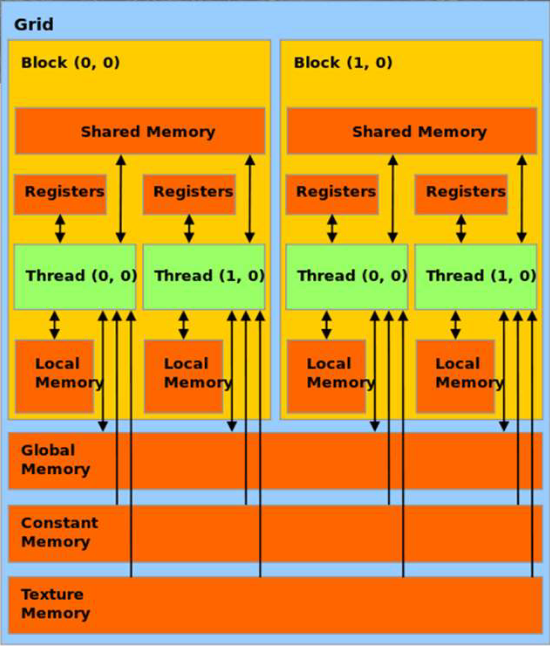
\includegraphics[width=0.7\linewidth]{img/type_of_memory.png}
    \caption{Tipi di memoria \cite{CUDAtutorial}}
\end{figure}


\subsection{Memoria condivisa (Shared Memory)}
La \textit{memoria condivisa} è una memoria veloce e a bassa latenza, accessibile da tutti i thread all'interno dello stesso blocco. È utile per condividere dati tra thread e ridurre l'accesso alla memoria globale, ottimizzando le prestazioni dei programmi paralleli. La memoria condivisa è limitata in quantità e deve essere gestita con attenzione.

\subsection{Memoria globale (Global Memory)}
La \textit{memoria globale} è la memoria principale accessibile da tutti i thread e blocchi. Essa ha una latenza elevata, quindi è preferibile minimizzarne l'utilizzo, soprattutto se si può sfruttare la memoria condivisa. Tuttavia, la memoria globale ha una capacità molto maggiore rispetto alla memoria condivisa.

\subsection{Memoria locale (Local Memory)}
La \textit{memoria locale} è assegnata ai singoli thread e viene utilizzata per memorizzare variabili private. Nonostante il nome, questa memoria è fisicamente una parte della memoria globale, e pertanto ha tempi di accesso relativamente lenti.

\subsection{Memoria costante (Constant Memory)}
La \textit{memoria costante} è una memoria a sola lettura che viene utilizzata per valori che rimangono invariati durante l'esecuzione di un kernel. Essendo memorizzata nella cache, ha una latenza più bassa rispetto alla memoria globale quando viene letta simultaneamente da più thread.

\subsection{Memoria di texture (Texture Memory)}
La \textit{memoria di texture} è progettata per il recupero efficiente di dati strutturati e può essere utilizzata per migliorare le prestazioni in applicazioni che richiedono accessi irregolari ai dati. Viene spesso usata in ambiti grafici, ma è accessibile anche per scopi generali.

\subsection{Registri}
I \textit{registri} sono la forma di memoria più veloce in CUDA e sono utilizzati per memorizzare variabili temporanee all'interno dei thread. Ogni thread ha accesso ai propri registri, che sono molto limitati in numero. Un uso inefficiente dei registri può portare al cosiddetto \textit{spill} nella memoria locale, con conseguente rallentamento delle prestazioni.







\chapter{Panoramica della localizzazione e mappatura simultanea (SLAM)}

\section{Introduzione al SLAM}

La Localizzazione e Mappatura Simultanea, comunemente nota come \textbf{SLAM} (\textit{Simultaneous Localization and Mapping}), rappresenta uno dei pilastri fondamentali della robotica moderna e della visione artificiale. SLAM si riferisce al processo computazionale mediante il quale un agente autonomo, come un robot o un veicolo, costruisce una mappa dell'ambiente circostante mentre contemporaneamente determina la propria posizione all'interno di essa.

\vspace{1cm}

\subsection{Importanza e applicazioni del SLAM}

L'importanza del SLAM risiede nella sua capacità di conferire autonomia a sistemi robotici in ambienti non strutturati o sconosciuti. Le applicazioni del SLAM sono molteplici e in rapida espansione:


\begin{enumerate}
    \item \textbf{Robotica mobile}: SLAM è essenziale per la navigazione autonoma di robot in ambienti interni ed esterni.
    \item \textbf{Veicoli autonomi}: Automobili e droni self-driving utilizzano tecniche SLAM per navigare in sicurezza.
    \item \textbf{Realtà aumentata (AR)}: SLAM permette il posizionamento accurato di oggetti virtuali nel mondo reale.
    \item \textbf{Esplorazione spaziale}: Robot su altri pianeti utilizzano SLAM per navigare e mappare terreni sconosciuti.
    \item \textbf{Ispezioni industriali}: SLAM facilita l'automazione di ispezioni in ambienti complessi come impianti industriali.
    \item \textbf{Servizi di emergenza}: Può assistere nelle operazioni di ricerca e salvataggio in aree disastrate.
\end{enumerate}

\subsection{Sfide principali nel campo del SLAM}

\begin{enumerate}
    \item \textbf{Incertezza e rumore}: I sensori non sono perfetti e introducono errori nelle misurazioni.
    \item \textbf{Ambienti dinamici}: Oggetti in movimento possono complicare la costruzione di mappe coerenti.
    \item \textbf{Loop closure}: Riconoscere luoghi già visitati è cruciale ma computazionalmente costoso.
    \item \textbf{Scalabilità}: Mantenere performance in tempo reale su mappe di grandi dimensioni.
    \item \textbf{Robustezza}: Garantire un funzionamento affidabile in condizioni ambientali variabili.
    \item \textbf{Efficienza computazionale}: Ottimizzare l'utilizzo delle risorse, specialmente su piattaforme con capacità limitate.
\end{enumerate}

\newpage

\subsection{Caratteristiche principali di ORB-SLAM}

\subsubsection{Rilevamento delle caratteristiche}
        Utilizza ORB (Oriented FAST and Rotated BRIEF) come descrittori di caratteristiche visive. Questi sono efficienti sia in termini di tempo di calcolo che di robustezza rispetto a variazioni di illuminazione e rotazioni.


\begin{figure}[h]
    \centering
    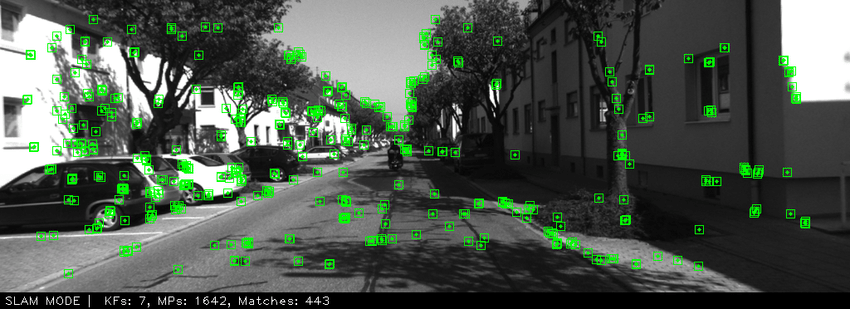
\includegraphics[width=1\linewidth]{img/ORB_SLAM2_feature.png}
    \caption{Ottenimento dei punti chiave in un frame \cite{SLAM2_Feature}}
\end{figure}


\subsubsection{Localizzazione e Mappatura}
        ORB-SLAM integra la localizzazione del dispositivo e la mappatura dell'ambiente in un unico framework. Utilizza le caratteristiche ORB estratte dalle immagini per stimare la posizione e orientamento della fotocamera mentre costruisce una mappa 3D dell'ambiente.



\subsubsection{Gestione delle chiavi e dei loop closure}
        Il sistema gestisce una mappa di punti chiave e riconosce i ritorni (\textbf{loop closures}) per correggere eventuali errori accumulati nella stima della posizione, migliorando così l'accuratezza della mappa e della localizzazione.

\begin{figure}[h]
    \centering
    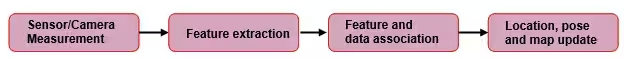
\includegraphics[width=1\linewidth]{img/SLAM_schema.jpg}
    \caption{Diagramma a blocchi generico e semplificato del processo SLAM basato sulle caratteristiche \cite{SLAM_algoritm2}}
    
\end{figure}

\subsubsection{Tracking, Mappatura e Rilevamento di Loop}
        ORB-SLAM divide il processo in tre thread principali: \textbf{tracking} (tracciamento della fotocamera), \textbf{mappatura} (costruzione e aggiornamento della mappa) e \textbf{rilevamento di loop} (riconoscimento di posizioni precedentemente visitate) con successiva chiusura del loop.

\begin{figure}[h]
    \centering
    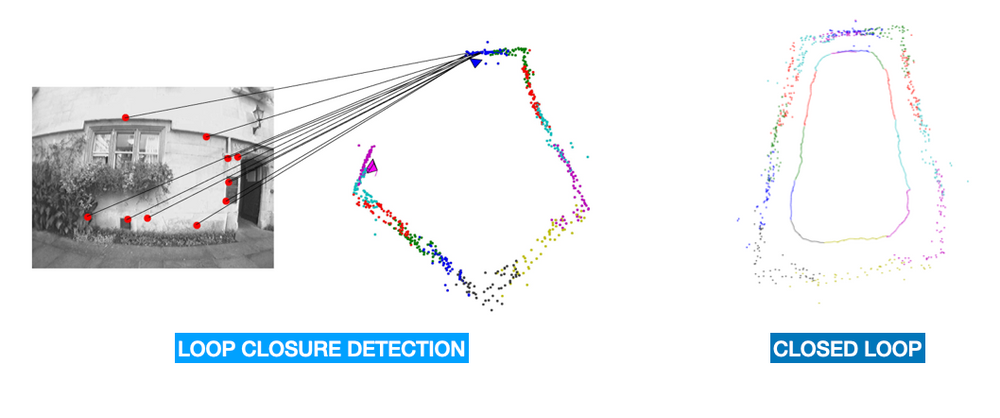
\includegraphics[width=1\linewidth]{img/loop_closure.png}
    \caption{Rappresentazione algoritmo di loop closure \cite{loop_closure}}
    
\end{figure}

\begin{figure}[h]
    \centering
    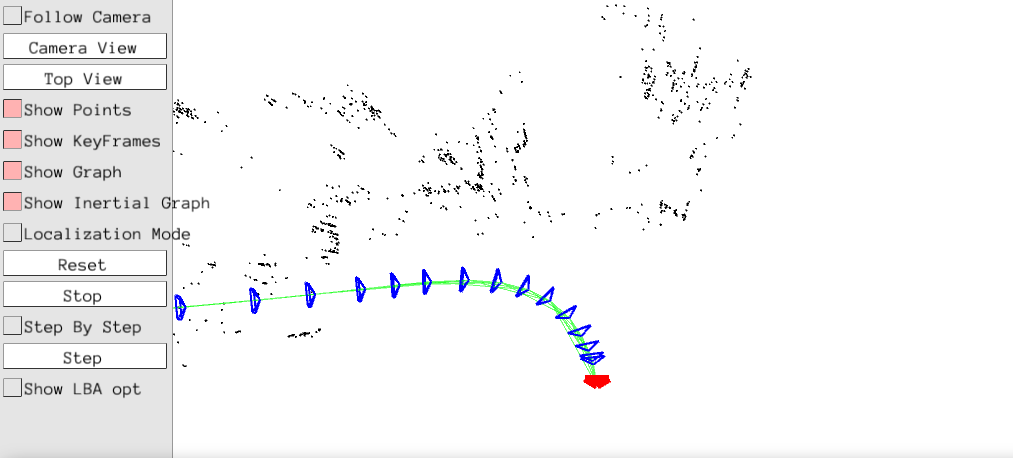
\includegraphics[width=1\linewidth]{img/map_viewer.png}
    \caption{"Cattura" dello schermo durante la generazione della mappa ambientale}
\end{figure}




\chapter{Analisi e scopo della ricerca}

\section{Introduzione}

L'obiettivo di questo capitolo è ottimizzare un algoritmo di \textbf{Stereo Matching} attraverso la parallelizzazione. In particolare, l'algoritmo contiene già una fase di estrazione \textit{ORB (Oriented FAST and Rotated BRIEF)} parallelizzata, ma vi sono ancora altre parti del processo che possono essere migliorate sfruttando la parallelizzazione.

\begin{figure}[h]
    \centering
    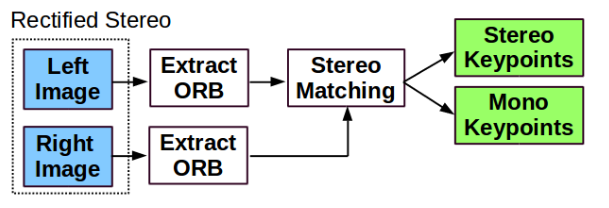
\includegraphics[width=0.7\linewidth]{img/start_point_opt.png}
    \caption{Stato iniziale del programma \cite{ORB_SLAM_2}}
\end{figure}


Per raggiungere questo obiettivo, il linguaggio di programmazione CUDA verrà utilizzato per implementare soluzioni che consentano di sfruttare le capacità di calcolo parallelo delle GPU, al fine di ridurre il tempo di elaborazione dell'algoritmo e migliorare le prestazioni complessive.
Nelle seguenti sezioni verrano mostrati i passaggi per la realizzazione del progetto.


\section{Installazione del sistema operativo}

Il sistema operativo scelto per il progetto è \textbf{Linux Mint 21.3}, è una distribuzione basata su \textit{Ubuntu} che offre un ambiente desktop intuitivo e facile da usare. Tra i vantaggi principali di Linux Mint e di Linux in generale troviamo la stabilità, la flessibilità, e una comunità di supporto attiva. \textit{Linux Mint}, in particolare, offre un'interfaccia utente simile a \textit{Windows}, rendendo la transizione semplice per gli utenti che non hanno familiarità con altri sistemi Linux.

\begin{figure}[h]
    \centering
    
\includegraphics[width=0.2\linewidth]{img/mint_logo.png}
    \caption{Linux Mint - Logo}
\end{figure}

Di seguito sono elencati i passaggi principali per l'installazione del sistema operativo:

\begin{enumerate}
    \item \textbf{Scaricare la distribuzione:} La distribuzione di Linux Mint 21.3 può essere scaricata direttamente dal sito ufficiale: \url{https://linuxmint.com/download.php}.
    \item \textbf{Creare una chiavetta USB avviabile:} Per scrivere l'immagine del sistema operativo su una chiavetta USB, è stato utilizzato un software come \textit{Rufus}. La chiavetta è stata preparata con una partizione di tipo GPT e con il file system NTFS per garantire la compatibilità.
    \item \textbf{Installazione in dual-boot:} L'installazione è stata effettuata in modalità \textit{dual-boot}, permettendo così di mantenere il sistema operativo preesistente insieme a Linux Mint. Il dual-boot è una configurazione che consente di scegliere quale sistema operativo avviare all'accensione del computer, garantendo la massima flessibilità nell'uso del dispositivo.
    \item \textbf{Modifica dell'ordine di boot:} Dopo aver creato la chiavetta USB, è stato necessario modificare l'ordine di avvio (boot) dal \textbf{BIOS/UEFI }del computer, per poi procedere con l'installazione definitiva di \textit{Linux Mint}.
\end{enumerate}


\section{Installazione ed avvio di ORB-SLAM 3}

In questo capitolo verrà descritta l'installazione e l'avvio del sistema ORB-SLAM3, uno dei più avanzati algoritmi di localizzazione e mappatura simultanea (SLAM). Verranno spiegati i passaggi principali necessari per configurare correttamente l'ambiente, installare le dipendenze e avviare ORB-SLAM3. L'obiettivo è fornire una guida dettagliata che permetta di eseguire l'algoritmo su un sistema basato su Linux, evidenziando eventuali problematiche comuni e come risolverle.

\subsection{Installazione del CUDA Toolkit}

Per poter sviluppare applicazioni con CUDA, è necessario installare il CUDA Toolkit, disponibile direttamente dal sito di NVIDIA. Questo toolkit contiene tutti gli strumenti necessari per la compilazione e l'esecuzione di codice parallelo su GPU, inclusi compilatori, librerie e campioni di codice. I passaggi principali necessari sono i seguenti e sono presi dal seguente tutorial \url{https://docs.nvidia.com/cuda/cuda-installation-guide-linux/index.html}

\begin{itemize}
    \item 1. Controllare la versione di CUDA con il comando \textbf{nvidia-smi}
    \item 2. Scaricare la versione di CUDA corrispondente alla versione restituita dal comando precedente. Example: 
    \begin{verbatim}
    Driver Version: 535.171.04   CUDA Version: 12.2
    \end{verbatim}
    
    \item 3. Aprire il file .bashrc e inserire il seguente comando:
    \begin{verbatim}
    export PATH=/usr/local/cuda-{version}/bin/:$PATH
    \end{verbatim}
\end{itemize}

\subsection{Ottenimento del Kitty Data Set}

Il \textbf{KITTI dataset} è un insieme di dati ampiamente utilizzato nella ricerca su visione artificiale e guida autonoma. È composto da immagini, informazioni di navigazione (GPS/IMU), e dati LiDAR raccolti da veicoli in ambienti urbani, utilizzato per allenare e valutare algoritmi come rilevamento di oggetti, segmentazione semantica, e SLAM (Simultaneous Localization and Mapping).

Per installarlo è sufficiente loggarsi sul sito \url{https://www.cvlibs.net/datasets/kitti/eval_odometry.php} e scaricare il pacchetto \textit{odometry data set (grayscale, 22 GB)}

\begin{figure}[h]
    \centering
    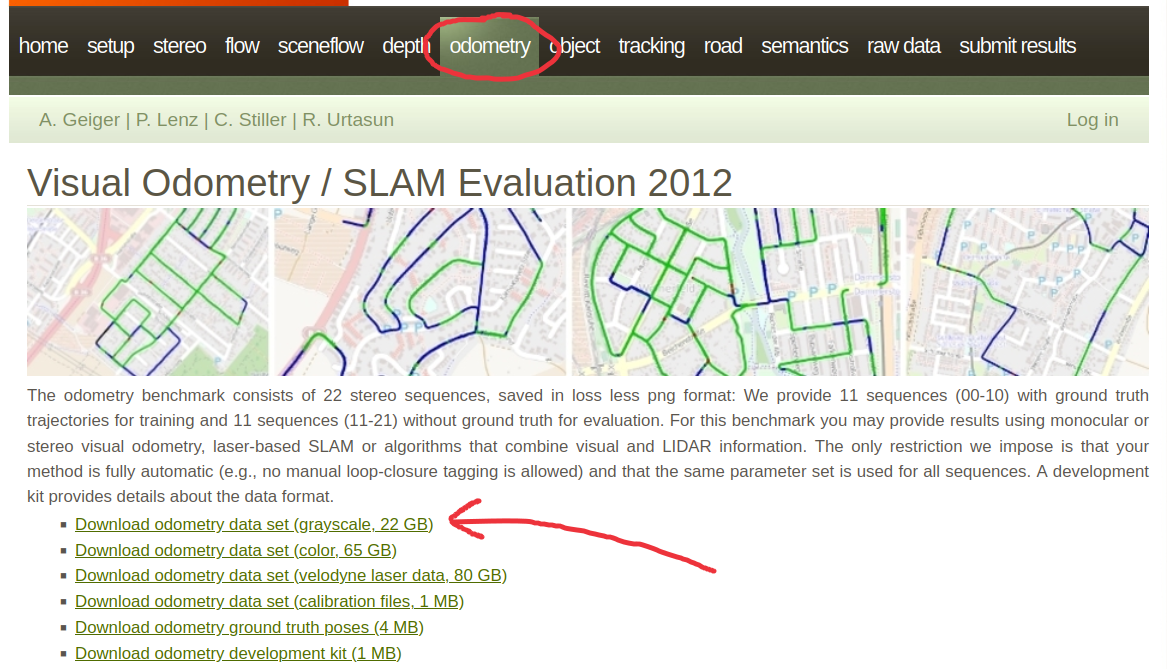
\includegraphics[width=0.9\linewidth]{img/kitti_dataset.png}
    \caption{Indicazione pacchetto da scaricare}
\end{figure}

\subsection{Installazione definitiva di ORB-SLAM3}

Per avvicinarci all'installazione finale di ORB-SLAM3 parallelo prima scarichiamo la versione non ottimizata, a seguire i passaggi descritti di seguito.

\begin{enumerate}
    \item \textbf{Clonare il repository:} Per prima cosa, clonare il repository di ORB-SLAM3 dal seguente URL: \url{https://github.com/UZ-SLAMLab/ORB_SLAM3}. Utilizzare il seguente comando nel terminale:

    \begin{verbatim}
    git clone https://github.com/UZ-SLAMLab/ORB_SLAM3.git
    \end{verbatim}

    \item \textbf{Eseguire la build:} Dopo aver clonato il repository, entrare nella directory di ORB-SLAM3 ed eseguire il processo di build con i comandi seguenti:

    \begin{verbatim}
    cd ORB_SLAM3
    chmod +x build.sh
    ./build.sh
    \end{verbatim}

    \item \textbf{Eseguire ORB-SLAM3:} Una volta completata la build, è possibile avviare ORB-SLAM3 con il comando seguente. Entrare nella directory principale di ORB-SLAM3 e utilizzare il comando:

    \noindent
    \begin{verbatim}
    
    ./Examples/Stereo/stereo_kitti Vocabulary/ORBvoc.txt 
    Examples/Stereo/KITTIX.yaml ~/Desktop/dataset/sequences/00
    \end{verbatim}

    Questo comando avvierà ORB-SLAM3 utilizzando il KITTI dataset per la modalità stereo.
    In base alla sequenza che andremo ad utilizzare bisogna cambiare \textbf{KITTIX.yaml} : 
    \begin{itemize}
        \item  KITTI00-02.yaml → sequenze 00,01,02.
        \item KITTY03.yaml → sequenze 03.
        \item KITTY04-12.yaml → sequenze 04,05,06,07,08,09,10,11,12.
    \end{itemize}
\end{enumerate}

\newline

Una volta che si è riusciti ad avviare la versione sopra citata, è possibile a passare alla versione parallela.
Infatti la versione attualmente in esecuzione, non è quella citata all'inizio del capitolo, questo perchè non contiene la parte di \textit{Estrazione ORB} parallelizata.
Per fare in modo di eseguire la versione in parallelo è necessario seguire i medesimi step con il seguente repository: \url{https://git.hipert.unimore.it/fmuzzini/cuda-accelerated-orb-slam}

\section{Analisi delle possibili ottimizazioni}

Durante l'analisi del codice di ORB-SLAM3, è stata individuata la funzione 
\begin{lstlisting}
void Frame::ComputeStereoMatches()}
\end{lstlisting} 
che si occupa dell'esecuzione della parte di \textbf{Stereo Matching}. 
Successivamente è stata eseguita una schematizzazione ed è stata analizzatata la sua struttura per identificare le possibili aree su cui intervenire per effettuare le ottimizzazioni.

\subsection{Schema generale}

Lo schema generale del funzionamento della funzione \texttt{ComputeStereoMatches()} è illustrato nell'immagine sottostante. Tale schema si compone di tre macro-funzioni principali e mostra il numero medio di iterazioni eseguite, permettendo di vedere il carico computazionale svolto.

\begin{figure}[h]
    \centering
    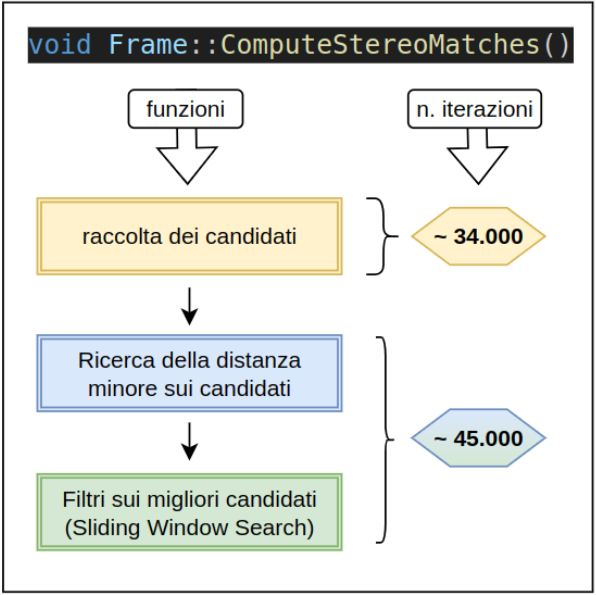
\includegraphics[width=0.8\linewidth]{img/ComputeStereo_schema.png}
    \caption{Schematizzazione della funzione \textit{ComputeStereoMatches()} }
\end{figure}

\begin{enumerate}
    \item \textbf{Raccolta dei keypoints:} La prima funzione si occupa di selezionare, per ogni punto chiave(keypoint) dell'immagine destra, un intorno e di aggiungerlo a una struttura dati apposita, preparandolo per le fasi successive.
    \item \textbf{Selezione del miglior candidato:} La seconda funzione si concentra sulla ricerca del miglior candidato tra quelli selezionati nella fase precedente, valutando i vari intorni e scegliendo quello più adatto.
    \item \textbf{Filtraggio dei risultati:} La terza funzione applica filtri ai keypoints migliori, al fine di mantenere solo quelli che soddisfano determinati criteri di qualità, migliorando così la precisione complessiva del processo.
\end{enumerate}

\newpage
\subsection{Schema della ricerca dei migliori candidati}

Nell'illustrazione sottostante è possibile visionare la schematizzazione della funzione addetta a trovare i migliori punti chiave tra quelli candidati (cioè quelli con distanza minore dall'immagine a sinistra)

Ci sono due tipi di rappresentazioni. Quella ad \textbf{alta livello} che è astratta e non tiene conto delle strutture dati. Mentre la seconda si concentra sulle \textbf{strutture dati utilizzate} e \textbf{le iterazioni} eseguite per raggiungere il risultato atteso.

\begin{figure}[h]
    \centering
    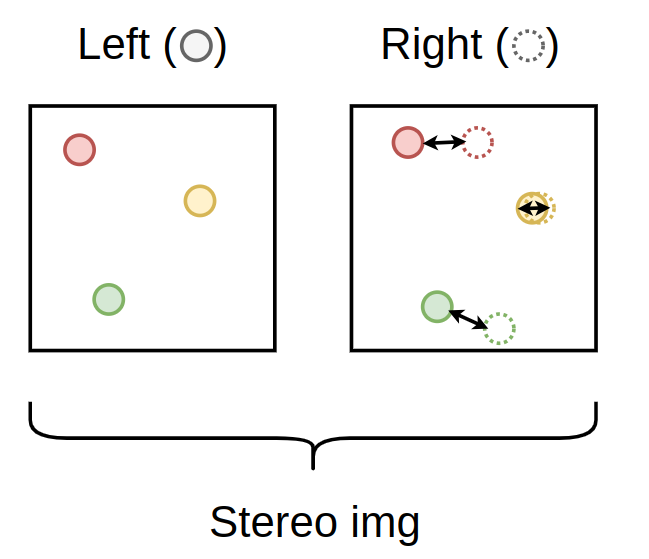
\includegraphics[width=0.5\linewidth]{img/find_distance_high_scheme.png}
    \caption{Schematizzazione ad alto livello (CPU) }
\end{figure}

Come si può vedere nell'immagine questa parte dell'algoritmo calcolerà la varie distanze, tra i punti \textbf{candidati trovati} ed i punti effettivi nell'\textbf{immagine sinistra}.
E successivamente andrà a scartare i candidati non ottimali.



\begin{figure}[H]
    \centering
    \fbox{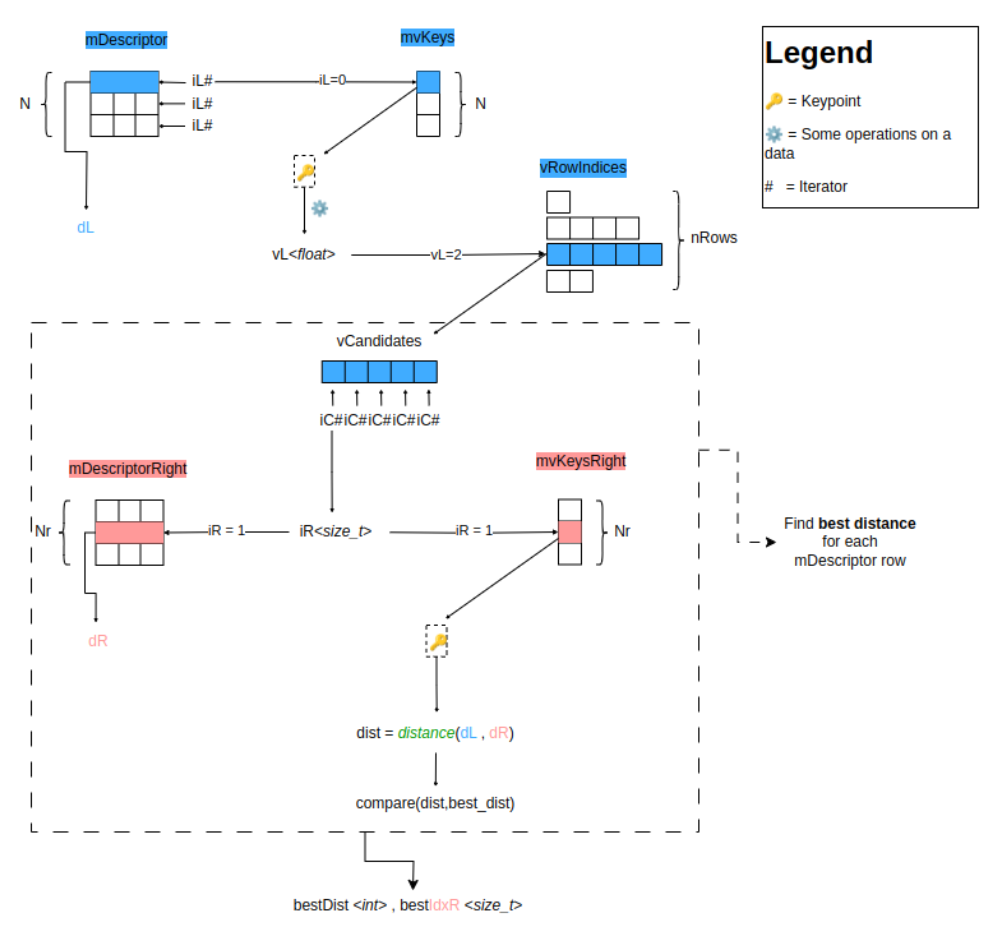
\includegraphics[width=1\textwidth]{img/find_best_distance.png}}
    \caption{Schematizzazione a basso livello (CPU) }
\end{figure}

\subsection{Parallelizzazione della ricerca dei migliori candidati}

\subsection{Schema del filtraggio finale sui punti chiave}

In questa sezione, analizzeremo il processo di Sliding Window nel contesto del nostro sistema ORB-SLAM 3 nella versiona non ottimizata per CPU. 

\begin{enumerate}
    \item L'immagine seguente illustra schematicamente la componente \textbf{Sliding Window} del sistema:
    
    \item È importante notare che il filtraggio associato alla Sliding Window viene eseguito successivamente al calcolo della distanza minore di un singolo punto chiave. Questo permette, eventualmente, di non attendere il calcolo di tutte le distanze ma di eseguire il filtraggio ad ogni singolo punto chiave.
\end{enumerate}

\begin{figure}[h]
    \centering
    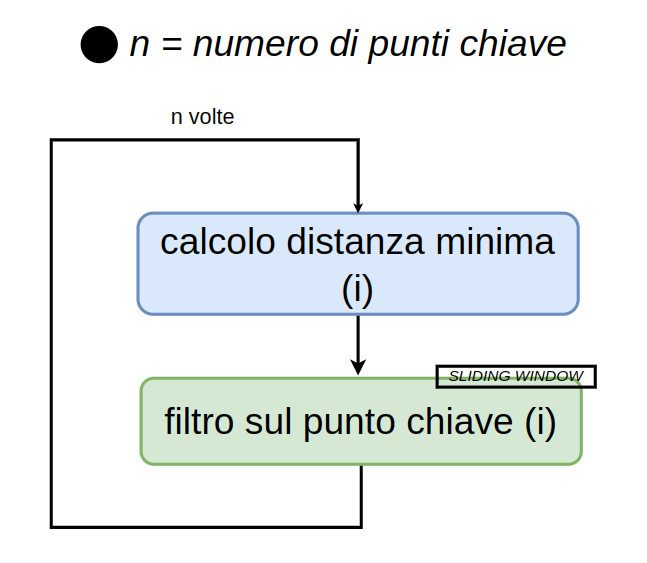
\includegraphics[width=0.6\textwidth]{img/sliding_window_high.png}
    \caption{Schematizzazione a basso livello (CPU) }
\end{figure}

\begin{figure}[h]
    \centering
    \fbox{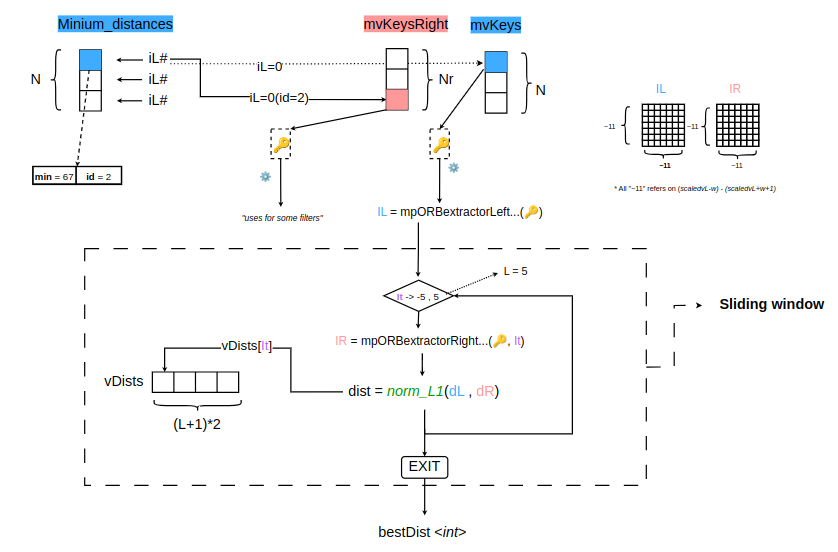
\includegraphics[width=1\textwidth]{img/sliding_window.png}}
    \caption{Schematizzazione a basso livello (CPU) }
\end{figure}


\chapter{Esperimenti e risultati}

\section{Introduzione agli esperimenti}

Nel contesto della nostra ricerca si è pensato di progettare una serie di esperimenti per valutare l'efficacia delle nostre modifiche. Questa sezione delinea la metodologia sperimentale, gli strumenti utilizzati e l'ambiente hardware in cui sono stati condotti gli esperimenti.

\subsection{Valutazione della Qualità}

La qualità degli esperimenti sarà valutata utilizzando un programma specializzato scritto in Python. Questo software è stato sviluppato specificamente per l'analisi e la valutazione di sistemi di odometria visiva e SLAM, con particolare attenzione alle prestazioni su dataset KITTI.

Il programma di valutazione è disponibile pubblicamente e può essere accessibile al seguente link:
\url{https://github.com/Huangying-Zhan/kitti-odom-eval}

\subsection{Ambiente Hardware e Software}

Gli esperimenti sono stati condotti su un sistema con le seguenti specifiche tecniche:

\begin{itemize}
    \item CPU: 12th Gen Intel(R) Core(TM) i7-1280P
    \item GPU: GeForce RTX 3060 Mobile / Max-Q , 6Gb
    \item RAM: 16 GB DDR4-3200
    \item Storage: 1 TB NVMe SSD
    \item Sistema Operativo: Linux mint 21.3
    \item CUDA Driver Version: 535.183.01  
    \item CUDA Version: 12.2
\end{itemize}

\subsection{Procedura Sperimentale}

Per eseguire gli esperimenti e la valutazione, seguire il seguente tutorial script:

\begin{enumerate}
    \item Spostarsi nella directory \texttt{/kitti-odom-eval}.
    \item Eseguire il comando: \verb|conda env update --file <nome_file.yml> --prune|
    \item Attivare l'ambiente conda con: \verb|conda activate kitti_eval|
    \item Spostare il file "CameraTrajectory.txt" nella directory \texttt{/result} e rinominarlo in "\texttt{<SEQ>.txt}" (Esempio: "07.txt").
    \item Eseguire il comando di valutazione: 
    \begin{verbatim}
    python3 eval_odom.py --result result --seqs <sequence> --align scale
    \end{verbatim}
\end{enumerate}

Questa procedura ci permetterà di valutare in modo consistente e riproducibile le prestazioni del nostro sistema ottimizzato, confrontandole con i risultati di riferimento del dataset KITTI.

Nei paragrafi seguenti, presenteremo i risultati ottenuti da questi esperimenti e discuteremo le implicazioni per il nostro lavoro di ottimizzazione.

\newpage
\section{Esperimento 1 - Variazione raggio dei candidati}

In questa fase del nostro studio, procederemo a modificare il parametro \textbf{radiusMultiplier}  della funzione che raccoglie i \textbf{candidati}. L'obiettivo è analizzare l'impatto di queste variazioni sulle prestazioni complessive del sistema. Nello specifico, valuteremo i potenziali vantaggi e svantaggi derivanti da ciascuna modifica, con particolare attenzione alle \textbf{implicazioni temporali}.

Qualora si riscontrino significativi aumenti nei tempi di elaborazione, considereremo l'opportunità di \textbf{ottimizzare il processo} mediante l'utilizzo di GPU. L'implementazione di soluzioni di calcolo parallelo su GPU potrebbe consentirci di mitigare gli effetti negativi osservati, sfruttando la capacità di elaborazione massiccia di queste unità hardware.

Il fine ultimo di questa analisi è individuare una configurazione ottimale che bilanci efficacemente la qualità dei risultati e l'efficienza computazionale. Attraverso questa metodologia di sperimentazione e ottimizzazione, miriamo a sviluppare \textbf{una versione migliorata del sistema}, che rappresenti un avanzamento significativo rispetto all'implementazione originale.

\vspace{1cm}

CODE : Codice relativo all'inserimento dei candidati
\begin{lstlisting}
for(int iR=0; iR<Nr; iR++){
    const cv::KeyPoint &kp = mvKeysRight[iR];
    const float &kpY = kp.pt.y;
    
    // Variabile modifica per esperimento
    const float radiusMultiplier = 2.0 
    const float r = radiusMultiplier *mvScaleFactors[mvKeysRight[iR].octave];  
    const int maxr = ceil(kpY+r);
    const int minr = floor(kpY-r);
    // Inserimento candidati nell'intorno del raggio
    for(int yi=minr;yi<=maxr;yi++){
        vRowIndices[yi].push_back(iR);
        size_refer[yi]++;   
    }
}
\end{lstlisting}

\vspace{4cm}

\subsection{Analisi dell'Impatto del parametro Radius: Risultati e Limiti}

L'esperimento condotto per valutare l'influenza del parametro 'radius' sulle prestazioni del sistema ORB-SLAM 3 ha portato a risultati che possiamo considerare positivi, soprattutto in termini di \textit{miglioramento della precisione}.

Le variazioni del valore del raggio in aumento, hanno prodotto dei miglioramenti termini di precisione per il valore ATE(m).

\begin{itemize}
    \item \textit{Kitti04 / Kitti07} : Miglioramento precisione ATE per un moltiplicatore di raggio pari a \textbf{16}.
    \item \textit{Kitti06} : Miglioramento precisione ATE per un moltiplicatore di raggio pari a \textbf{4}.
\end{itemize}

l'\textbf{ATE} (Absolute Trajectory Error) è una misura utilizzata per valutare la precisione della traiettoria stimata dal sistema di SLAM rispetto alla traiettoria di riferimento (ground truth).

Si osserva inoltre che i tempi nella parte di \textbf{Stereo Matching} mostrano un aumento significativo, con incrementi che arrivano fino al 100\%. Si può prevedere che questo problema diventi trascurabile con la parallelizzazione dell'algoritmo. L'aumento dei tempi di elaborazione, infatti, potrà essere mitigato sfruttando l'elaborazione parallela, consentendo di distribuire il carico computazionale e ridurre significativamente i tempi complessivi.



\begin{table}[h]
    \centering
    \caption{Esperimenti variazione raggio (KITTY DATASET - 04) }
    \begin{tabular}{lcccccc}
        \toprule
        \rowcolor{gray!20}
        Radius multiplier & 1.0 & \cellcolor{orange!40}2.0 & 4.0 & 8.0 & 16.0 \\
        \midrule
        %%%
        Translation error & 0.47 & \cellcolor{green!20}0.46 & \cellcolor{green!20}0.46 & 0.47 & 0.47 \\
        %%%
        Rotational error  & \cellcolor{green!20}0.07 & 0.08 & 0.09 & \cellcolor{green!20}0.07 & \cellcolor{green!20}0.07 \\
        %%%
        ATE (m)           & 0.73 & 0.77 & 0.75 & 0.78 & \cellcolor{green!20}0.71 \\
        %%%
        RPE (m)           & \cellcolor{green!20}0.017 & \cellcolor{green!20}0.017 & \cellcolor{green!20}0.017 & \cellcolor{green!20}0.017 & \cellcolor{green!20}0.017 \\
        %%%
        RPE (deg)         & 0.031 & 0.032 & 0.031 & \cellcolor{green!20}0.030 & \cellcolor{green!20}0.030 \\
        %%%
        ORB Extraction (ms) & 9.1419 & \cellcolor{green!20}8.9207 & \cellcolor{green!20}8.9707 & 9.0029 & 8.9305 \\
        %%%
        Stereo Matching (ms) & \cellcolor{green!20}3.0216 & 3.391 & 3.962 & 4.8351 & 6.345 \\
        %%%
        ORB Extraction ($\sigma$) & 61.54 & \cellcolor{green!20}57.737 & 58.214 & 58.98 & 58.148 \\
        %%%
        Stereo Matching ($\sigma$) & \cellcolor{green!20}0.54303 & 0.63088 & 0.68821 & 0.74869 & 0.6854 \\
        \bottomrule
    \end{tabular}
\end{table}


\begin{table}[h]
    \centering
    \caption{Esperimenti variazione raggio (KITTY DATASET - 06) }
    \begin{tabular}{lcccccc}
        \toprule
        \rowcolor{gray!20}
        Radius multiplier & 1.0 & \cellcolor{orange!40}2.0 & 4.0 & 8.0 & 16.0 \\
        \midrule
        %%%
        Translation error & 0.48 & 0.48 & \cellcolor{green!20}0.46 & 0.48 & 0.48 \\
        %%%
        Rotational error & \cellcolor{green!20}0.15 & 0.16 & \cellcolor{green!20}0.15 & 0.16 & \cellcolor{green!20}0.15 \\
        %%%
        ATE (m)           & 2.43 & 2.45 & \cellcolor{green!20}2.29 & 2.59 & 2.31 \\
        %%%
        RPE (m)           & \cellcolor{green!20}0.013 & \cellcolor{green!20}0.013 & 0.014 & 0.014 & 0.014 \\
        %%%
        RPE (deg)         & \cellcolor{green!20}0.031 & \cellcolor{green!20}0.031 & 0.032 & 0.032 & 0.032 \\
        %%%
        ORB Extraction (ms) & 6.0595 & 6.0632 & \cellcolor{green!20}6.0573 & 6.0988 & 6.1996 \\
        %%%
        Stereo Matching (ms) & 2.832 & 3.231 & 3.732 & 4.678 & 6.281 \\
        %%%
        ORB Extraction ($\sigma$) & 28.606 & \cellcolor{green!20}28.451 & 28.551 & 28.839 & 28.839 \\
        %%%
        Stereo Matching ($\sigma$) & \cellcolor{green!20}0.534 & 0.557 & 0.645 & 0.716 & 0.681 \\
        \bottomrule
    \end{tabular}
\end{table}

\newpage
\begin{table}[h]
    \centering
    \caption{Esperimenti variazione raggio (KITTY DATASET - 07) }
    \begin{tabular}{lcccccc}
        \toprule
        \rowcolor{gray!20}
        Radius multiplier & 1.0 & \cellcolor{orange!40}2.0 & 4.0 & 8.0 & 16.0 \\
        \midrule
        %%%
        Translation error & 0.48 & \cellcolor{green!20}0.44 & 0.47 & 0.46 & 0.47 \\
        %%%
        Rotational error  & 0.24 & \cellcolor{green!20}0.23 & 0.25 & 0.26 & 0.26 \\
        %%%
        ATE (m)           & 0.52 & 0.49 & 0.5 & 0.54 & \cellcolor{green!20}0.46 \\
        %%%
        RPE (m)           & 0.014 & \cellcolor{green!20}0.013 & 0.014 & 0.014 & 0.014 \\
        %%%
        RPE (deg)         & 0.04 & \cellcolor{green!20}0.039 & 0.041 & 0.040 & 0.040 \\
        %%%
        ORB Extraction (ms) & 6.305 & 6.3717 & 6.356 & \cellcolor{green!20}6.280 & 6.679 \\
        %%%
        Stereo Matching (ms) & \cellcolor{green!20}3.087 & 3.573 & 4.072 & 4.896 & 6.679 \\
        %%%
        ORB Extraction ($\sigma$) & 29.31 & \cellcolor{green!20}28.58 & 29.45 & 28.65 & 29.87 \\
        %%%
        Stereo Matching ($\sigma$) & 0.535 & \cellcolor{green!20}0.526 & 0.642 & 0.689 & 0.688 \\
        \bottomrule
    \end{tabular}
\end{table}

Nella sezione successiva analizzeremo i risultati ottenuti in termini di tempi di esecuzione a seguito della parallelizazione  dell'algoritmo. Questo potrebbe offrire miglioramenti significativi sia in termini di efficienza e permettere un miglioramento della precisione senza perdite di prestazioni.


\newpage
\section{Esperimento 2 - Parallelizazione: ricerca delle distanze minime e filtraggio}

In questo capitolo, presenteremo il secondo esperimento condotto nell'ambito della nostra ricerca sull'ottimizzazione. L'obiettivo principale di questo esperimento è stato quello di parallelizzare due \textit{fasi critiche del nostro algoritmo}:

\begin{itemize}
    \item La ricerca delle distanze minime
    \item Il successivo processo di filtraggio
\end{itemize}

Attraverso questa parallelizzazione, ci proponiamo di sfruttare appieno le capacità di elaborazione parallela offerte dalle GPU, con l'intento di ottenere un significativo miglioramento delle prestazioni rispetto all'implementazione sequenziale.
Nel corso di questo capitolo, esamineremo in dettaglio:

\begin{enumerate}
    \item Gli step eseguiti per implementare la parallelizzazione.
    \item I risultati ottenuti dall'esperimento.
    \item Un'analisi comparativa delle prestazioni tra l'implementazione sequenziale e quella parallela.
\end{enumerate}

Questa esplorazione ci permetterà di valutare l'efficacia dell'approccio adottato e di trarre conclusioni sulle potenzialità dell'ottimizzazione in questo contesto specifico.

\begin{figure}[h]
    \centering
    \fbox{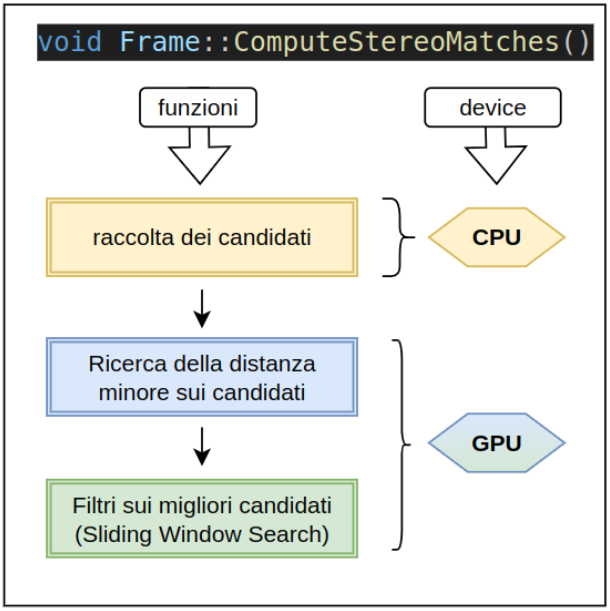
\includegraphics[width=0.5\textwidth]{img/experiment2_schema.png}}
    \caption{Distribuzione delle funzioni su device}
\end{figure}

\subsection{Avvicinamento alla soluzione}

Nel percorso verso la realizzazione del nostro obiettivo finale, si è ritenuto opportuno sviluppare un programma intermedio. Questo approccio ha permesso di affrontare gradualmente la complessità del problema, fornendo preziosi spunti e una base solida su cui costruire.
È importante sottolineare che questo programma intermedio, pur condividendo alcune similitudini con il nostro obiettivo finale, presenta delle differenze significative:

\begin{figure}[h]
    \centering
    \fbox{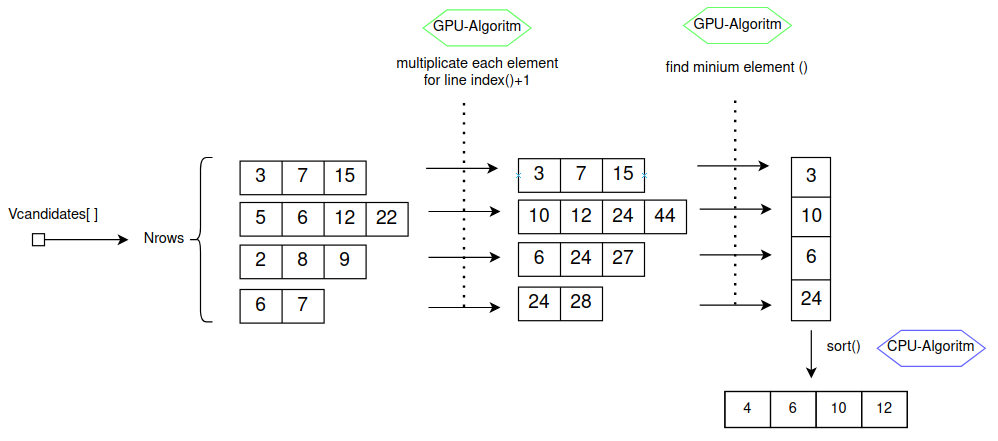
\includegraphics[width=1\textwidth]{img/opt1_simulation.png}}
    \caption{Schemattizazione del programma di "avvicinamento"}
\end{figure}

\vspace{2cm}

\subsection{Parallelizazione della "ricerca delle distanze minime" } \label{distanze-minime-gpu}

Per implementare la parallelizzazione della funzione di ricerca delle distanze minime, abbiamo seguito un approccio strutturato che ha richiesto la creazione di nuovi file e la modifica di quelli esistenti. Di seguito, descriviamo i passaggi principali di questo processo:

\subsubsection{Creazione di nuovi file}
Il primo passo è stato la creazione di due nuovi file:

\begin{itemize}
    \item \texttt{gpu\_stereoMatches.cu}: Questo file conterrà il codice CUDA per la parallelizzazione della funzione.
    \item \texttt{gpu\_stereoMatches.h}: Il file header corrispondente, che conterrà le dichiarazioni delle funzioni e le strutture dati necessarie.
\end{itemize}

In questi file, abbiamo implementato la logica per la parallelizzazione della ricerca delle distanze minime, sfruttando le capacità di elaborazione parallela offerte dalle GPU.

\subsubsection{Aggiornamento del CMakeLists.txt}

Per assicurarci che i nuovi file fossero inclusi correttamente nel processo di compilazione, abbiamo aggiunto le seguenti righe al file \texttt{CMakeLists.txt}:

\begin{verbatim}
src/gpu_stereoMatches.cu
include/gpu_stereoMatches.h
\end{verbatim}

Questa modifica garantisce che il compilatore riconosca e includa i nostri nuovi file CUDA durante il processo di build.

\subsubsection{Inclusione dell'header nel file Frame.cc}
Per rendere le nuove funzionalità accessibili all'interno del nostro framework esistente, abbiamo aggiunto la seguente linea di inclusione nel file \texttt{Frame.cc}:

\begin{verbatim}
#include "gpu_stereoMatches.h"
\end{verbatim}

Questo passaggio assicura che le funzioni e le strutture dati definite nei nostri nuovi file siano disponibili per l'uso all'interno del contesto del frame.

\subsubsection{Progettazione della struttura del kernel}
Dopo aver preparato l'infrastruttura necessaria, ci siamo concentrati sulla progettazione della struttura del kernel CUDA da lanciare. Questa fase ha comportato:

\begin{itemize}
\item L'analisi dell'algoritmo di ricerca delle distanze minime per identificare le parti parallelizzabili.
\item La definizione della griglia e dei blocchi di thread per ottimizzare l'esecuzione sulla GPU.
\item La progettazione delle funzioni del kernel per sfruttare efficacemente l'architettura parallela della GPU.
\end{itemize}

La struttura del kernel è stata progettata per massimizzare il parallelismo, permettendo l'elaborazione simultanea di molteplici punti di interesse e riducendo significativamente il tempo di esecuzione complessivo dell'algoritmo di ricerca delle distanze minime.

\vspace{1cm}

\begin{figure}[h]
    \centering
    \fbox{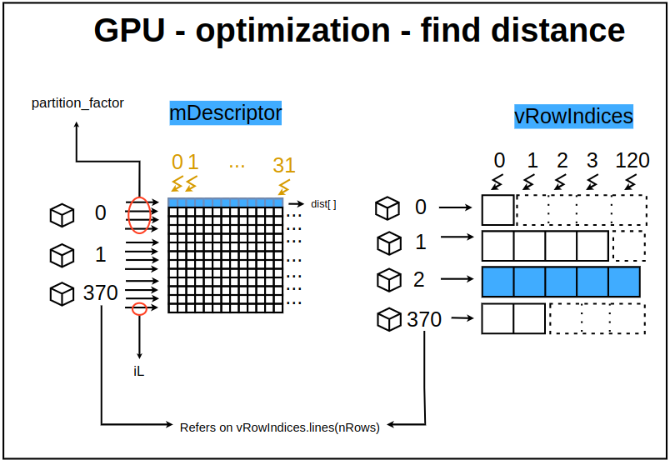
\includegraphics[width=0.6\textwidth]{img/GPU_opt1_findDistance.png}}
    \caption{Configurazione della griglia (calcolo distanza) }
\end{figure}

\begin{figure}[h]
    \centering
    \fbox{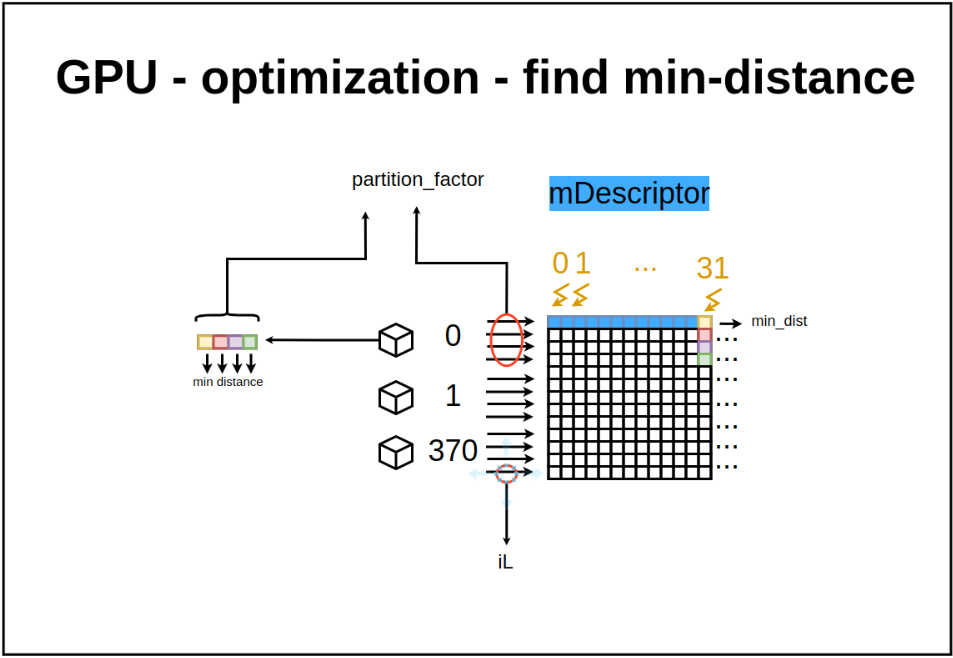
\includegraphics[width=0.6\textwidth]{img/GPU_opt1_findMinDistance.png}}
    \caption{Configurazione della griglia (calcolo distanza minima) }
\end{figure}

\subsubsection{Riscrittura funzione sequenziale (Distanza di Hamming) }

Abbiamo modificato la funzione che calcola la distanza di Hamming in modo che potesse essere chiamata direttamente dalla GPU. Questo è stato realizzato convertendo la funzione in una funzione di tipo \textbf{\_\_device\_\_}. Tale modifica permette alla funzione di essere eseguita direttamente sul dispositivo GPU, ottimizzando così le prestazioni e riducendo la necessità di trasferimenti di dati tra CPU e GPU.

\vspace{1cm}

CODE : Algoritmo per calcolare distanza di Hamming
\begin{lstlisting}
__device__ int DescriptorDistance(const unsigned char *a, const unsigned char* b){

    int dist=0;

    const int32_t* a_int = reinterpret_cast<const int32_t*>(a);
    const int32_t* b_int = reinterpret_cast<const int32_t*>(b);

    for(int i=0; i<8; i++) {
        unsigned int v = a_int[i] ^ b_int[i];
        v = v - ((v >> 1) & 0x55555555);
        v = (v & 0x33333333) + ((v >> 2) & 0x33333333);
        dist += (((v + (v >> 4)) & 0xF0F0F0F) * 0x1010101) >> 24;
    }

    return dist;
}
\end{lstlisting}


\subsubsection{Confronto precisione risultati}

\begin{figure}[h]
    \centering
    \fbox{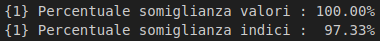
\includegraphics[width=1\textwidth]{img/minium_distance_accuracy.png}}
    \caption{Risultato accuratezza dell'algoritmo}
\end{figure}

\subsection{Parallelizazione del "filtraggio delle distanze" }

In questa parte dell'esperimento, abbiamo utilizzato i file configurazione del programma citati nella sezione precedente \ref{distanze-minime-gpu}. Questo approccio ci ha permesso di mantenere una coerenza metodologica e di costruire sulla base delle conoscenze già acquisite. Tuttavia, la differenza sostanziale in questa fase è stata l'introduzione di una nuova funzione di tipo \textbf{kernel()}, specifica per l'implementazione CUDA.
\subsubsection{Configurazione del programma}

\begin{enumerate}
    \item \texttt{gpu\_stereoMatches.cu}: Contenente il codice CUDA per la parallelizzazione.
    \item \texttt{gpu\_stereoMatches.h}: Il file header corrispondente.
\end{enumerate}

\vspace{1cm}

\subsubsection{Progettazione della struttura del kernel}

A seguito è stata progettata la \textbf{configurazione della griglia} in modo tale da sfruttare
a pieno il parallelismo e minimizzare l'utilizzo di registri della GPU.

\begin{figure}[h]
    \centering
    \fbox{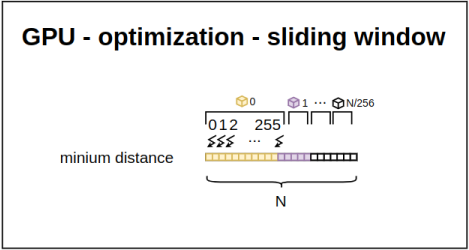
\includegraphics[width=0.7\textwidth]{img/GPU_opt1_slidingWindow.png}}
    \caption{Configurazione della griglia(sliding window) }
\end{figure}

\newpage
\subsubsection{Riscrittura funzione sequenziale (Norma Manhattan)}

Abbiamo riscritto la funzione che calcola la norma 1, nota anche come "distanza di Manhattan". Questa funzione, che nel programma CPU originale era stata implementata utilizzando la libreria OpenCV, è stata riscritta come una funzione di tipo \textbf{\_\_device\_\_}.

\begin{lstlisting}
__device__ float norm1(const uchar *V1 , const uchar* V2 , int size , int i1 , int j1 , int i2 , int j2 , int cols1 , int cols2 , int incR , int iL){

    float sum = 0;
    int countRow = 0;
    int countCol = 0;
    int j1_temp = j1;
    int j2_temp = j2;
    while(countRow < size){
        while(countCol < size){
            int index1 = ( (i1*cols1) + j1 );
            int index2 = ( (i2*cols2) + j2 );
            sum = sum + abs(((float) V1[index1] - (float) V2[index2]));
            countCol++;
            j1++;
            j2++;
        }
        i1++;
        i2++;
        j1 = j1_temp;
        j2 = j2_temp;
        countCol = 0;
        countRow++;
    }

    return sum;
    
}
\end{lstlisting}

\vspace{1cm}

È importante ricordare la definizione di norma 1 e il suo scopo: la norma 1, anche nota come distanza di Manhattan o distanza cityblock, è definita come la somma dei valori assoluti delle differenze delle coordinate. Nel nostro contesto, viene utilizzata per misurare la dissimilarità tra due vettori di caratteristiche, fornendo una metrica robusta per confrontare descrittori di immagini e identificare corrispondenze tra punti di interesse.

\begin{figure}[h]
    \centering
    \fbox{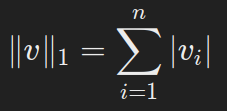
\includegraphics[width=0.4\textwidth]{img/norm1.png}}
    \caption{Definizione della Norma di Manhattan}
\end{figure}

\subsubsection{Confronto precisione risultati}

\begin{figure}[h]
    \centering
    \fbox{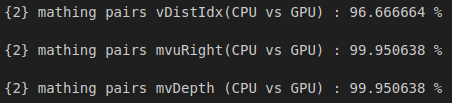
\includegraphics[width=1\textwidth]{img/sliding_window_accuracy.png}}
    \caption{Risultato accuratezza dell'algoritmo}
\end{figure}

\newpage
\subsection{Analisi dell'ottimizazione : Risultati e Conclusioni}

\subsubsection{Risultati}

\begin{table}[h]
    \centering
    \caption{Esperimenti variazione raggio (KITTY DATASET - 04) }
    \begin{tabular}{lcccccc}
        \toprule
        \rowcolor{gray!20}
        Device & \cellcolor{blue!20}GPU & \cellcolor{orange!20}CPU  \\
        \midrule
        %%%
        Translation error & \cellcolor{green!20}0.410 & 0.450  \\
        %%%
        Rotational error  & \cellcolor{green!20}0.220 & \cellcolor{green!20}0.220  \\
        %%%
        ATE (m)           & 0.610 & \cellcolor{green!20}0.480  \\
        %%%
        RPE (m)           & \cellcolor{green!20}0.014 & 0.015  \\
        %%%
        RPE (deg)         & \cellcolor{green!20}0.041 & 0.042  \\
        %%%
        ORB Extraction (ms) & \cellcolor{green!20}5.108 & 5.123  \\
        %%%
        Stereo Matching (ms) & 3.302 & \cellcolor{green!20}\textbf{0.939} && $\xleftarrow{}$ miglioramento (351\%) \\
        %%%
        ORB Extraction ($\sigma$) & 3.425 & \cellcolor{green!20}3.388  \\
        %%%
        Stereo Matching ($\sigma$) & 0.595 & \cellcolor{green!20}\textbf{0.117} && $\xleftarrow{}$ miglioramento (508\%)\\
        \bottomrule
    \end{tabular}
\end{table}

\vspace{1cm}

\begin{table}[h]
    \centering
    \caption{Esperimenti variazione raggio (KITTY DATASET - 06) }
    \begin{tabular}{lcccccc}
        \toprule
        \rowcolor{gray!20}
        Device & \cellcolor{blue!20}GPU & \cellcolor{orange!20}CPU  \\
        \midrule
        %%%
        Translation error & \cellcolor{green!20}0.670 & 0.690  \\
        %%%
        Rotational error  & \cellcolor{green!20}0.300 & 0.360  \\
        %%%
        ATE (m)           & \cellcolor{green!20}4.510 & 4.850  \\
        %%%
        RPE (m)           & \cellcolor{green!20}0.014 & 0.015  \\
        %%%
        RPE (deg)         & \cellcolor{green!20}0.033 & 0.034  \\
        %%%
        ORB Extraction (ms) & \cellcolor{green!20}4.729 & 4.768 &&  \\
        %%%
        Stereo Matching (ms) & 3.089 & \cellcolor{green!20}\textbf{0.947} & $\xleftarrow{}$ miglioramento (326\%) \\
        %%%
        ORB Extraction ($\sigma$) & 3.580 & \cellcolor{green!20}3.399  \\
        %%%
        Stereo Matching ($\sigma$) & 0.553 & \cellcolor{green!20}\textbf{0.124} & $\xleftarrow{}$ miglioramento (445\%) \\
        \bottomrule
    \end{tabular}
\end{table}

\begin{figure}[H]
    \centering
    \fbox{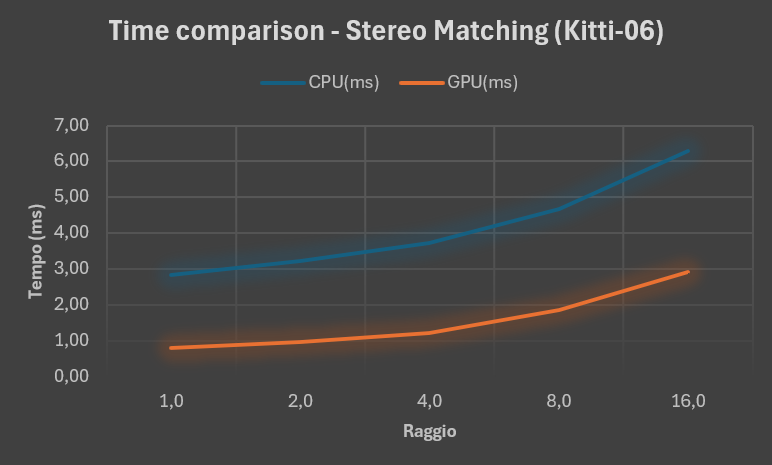
\includegraphics[width=1\textwidth]{img/time_comparison1_kitti06.png}}
    \caption{Comparazione dei tempi sull'algoritmo di Stereo Matching }
\end{figure}

\begin{table}[h]
    \centering
    \caption{Esperimenti variazione raggio (KITTY DATASET - 07) }
    \begin{tabular}{lcccccc}
        \toprule
        \rowcolor{gray!20}
        Device & \cellcolor{blue!20}GPU & \cellcolor{orange!20}CPU  \\
        \midrule
        %%%
        Translation error & 0.540 & \cellcolor{green!20}0.480  \\
        %%%
        Rotational error  & \cellcolor{green!20}0.110 & 0.130  \\
        %%%
        ATE (m)           & 0.700 & \cellcolor{green!20}0.630  \\
        %%%
        RPE (m)           & \cellcolor{green!20}0.017 & \cellcolor{green!20}0.017  \\
        %%%
        RPE (deg)         & 0.034 & \cellcolor{green!20}0.032  \\
        %%%
        ORB Extraction (ms) & \cellcolor{green!20}5.520 & 5.524 &&  \\
        %%%
        Stereo Matching (ms) & 3.284 & \cellcolor{green!20}\textbf{0.969}  & $\xleftarrow{}$ miglioramento (338\%)\\
        %%%
        ORB Extraction ($\sigma$) & 6.911 & \cellcolor{green!20}6.841  \\
        %%%
        Stereo Matching ($\sigma$) & 0.545 & \cellcolor{green!20}\textbf{0.130} & $\xleftarrow{}$ miglioramento (420\%) \\
        \bottomrule
    \end{tabular}
\end{table}



\newpage

\subsubsection{Conclusioni}

La parallelizzazione ha portato a un notevole incremento delle prestazioni in termini di tempo di esecuzione. Nello specifico, abbiamo osservato:
\begin{itemize}
\item Un incremento della velocità di esecuzione di oltre il \textbf{300\% }rispetto all'implementazione originale su CPU.
\item Una stabilità nella \textbf{precisione dei dati}, l'accuratezza è rimasta pressochè invariata.
\end{itemize}
Questo significativo aumento di efficienza dimostra il potenziale della computazione parallela su GPU per questo tipo di algoritmi di ricerca intensiva.



\subsubsection{Possibili ottimizazioni future}

Il notevole guadagno in termini di prestazioni offre l'opportunità di aumentare la complessità computazionale in futuro. Questo potrebbe permettere di ottenere risultati ancora più precisi senza compromettere le prestazioni complessive del sistema in termini di \textit{precisione} e \textit{tempo}. Ad esempio:
\begin{itemize}
\item Potremmo aumentare il numero di punti di interesse analizzati.
\item Potremmo implementare algoritmi di matching più sofisticati e computazionalmente intensivi.
\item Potremmo estendere l'analisi a più frame o a risoluzioni di immagine più elevate.
\end{itemize}



\chapter{Conclusioni}

// WRITE YOUR CONCLUSION...


\bibliographystyle{apalike}
\bibliography{bibliografia}  % type -> @online,@misc,@unpublished,@thesis,@article,@book,...

\end{document}


